\documentclass[nooutcomes]{ximera}
\usepackage{booktabs}
%% handout
%% space
%% newpage
%% numbers
%% nooutcomes

\renewcommand{\outcome}[1]{\marginpar{\null\vspace{2ex}\scriptsize\framebox{\parbox{0.75in}{\begin{raggedright}\textbf{P\arabic{problem} Outcome:} #1\end{raggedright}}}}}

\renewenvironment{freeResponse}{
\ifhandout\setbox0\vbox\bgroup\else
\begin{trivlist}\item[\hskip \labelsep\bfseries Solution:\hspace{2ex}]
\fi}
{\ifhandout\egroup\else
\end{trivlist}
\fi}

\newcommand{\RR}{\mathbb R}
\renewcommand{\d}{\,d}
\newcommand{\dd}[2][]{\frac{d #1}{d #2}}
\renewcommand{\l}{\ell}
\newcommand{\ddx}{\frac{d}{dx}}
\everymath{\displaystyle}
\newcommand{\dfn}{\textbf}
\newcommand{\eval}[1]{\bigg[ #1 \bigg]}


\title{Breakout Session 5 Solutions}  

\begin{document}
\begin{abstract}
  % \textbf{A look back:} In the previous (January 21, 2016) Breakout Session you practiced the fundamental techniques of evaluating limits using pen and paper.
  % Evaluating limits ``by hand'' essentially consists of two components: identifying the form of the limit and reshaping to transform a harder limit to an easier limit.

  % \textbf{Overview:} In today's (January 26, 2016) Breakout Session you will practice evaluating limits to locate horizontal and vertical asymptotes.
  % This skill also consists of two components: identifying the form of the limit and using the form to determine rapid growth, rapid decay, or end behavior.

  % \textbf{A look ahead:} In the next (January 28, 2016) Breakout Session you will investigate a special class of functions defined in terms of limits.
\end{abstract}
\maketitle

% \section{Learning Outcomes}
% \label{section:learning-outcomes}
% The following outcomes are \emph{not an exhaustive} list of the skills you will need to develop and integrate for demonstration on quizzes and exams.
% This list is meant to be a starting point for conversation (with your Lecturer, Breakout Session Instructor, and fellow learners) for organizing your knowledge and monitoring the development of your skills.

% % \subsection*{Outcomes for infinite limits}
% % \label{section:learning-outcomes-infinite-limits}
% \begin{itemize}
%   \item 
%     Recognize when a limit is indicating there is a vertical asymptote.

%   \item
%     Evaluate the limit as $x$ approaches a point where there is a vertical asymptote.

%   \item
%     Match graphs of functions with their equations based on vertical asymptotes.

%   \item  
%     Discuss what it means for a limit to equal $\pm\infty$.

%   \item 
%     Define a vertical asymptote.

%   \item
%     Understand the relationship between limits and vertical asymptotes.
% \end{itemize}

% % \subsection*{Outcomes for limits at infinity} 
% \begin{itemize}
%   \item
%     Calculate the limit as $x$ approaches $\pm\infty$ of common functions algebraically.

%   \item
%     Decide whether a form is determinate or indeterminate. 

%   \item
%     Find the limit as $x$ approaches $\pm\infty$ from a graph. 

%   \item 
%     Discuss why infinity is not a number. 
% \end{itemize}
% \newpage

\begin{problem}
  \label{problem:warmup-for-forms}
  \outcome{Recognize when a limit is indicating there is a vertical asymptote.}
  \outcome{Evaluate the limit as $x$ approaches a point where there is a vertical asymptote.}
  \outcome{Discuss what it means for a limit to equal $\pm\infty$.}
  \outcome{Understand the relationship between limits and vertical asymptotes.}
  \outcome{Decide whether a form is determinate or indeterminate.}
  For each of the following statements, produce a function $f$ such that it satisfies the stated conditions.
  \begin{itemize}
    \item[(a)]
      The limit of $f$ as $x$ approaches 4 has the form $\frac{0}{0}$ and the limit exists as a finite number, that is, 
      \[
        \lim_{x \to 4} \underbrace{f(x)}_{\text{form $0/0$}} = L,
      \]
      where $L$ is a real number.
      \begin{freeResponse}
        We have
        \begin{align*}
          \lim_{x \to 4} \underbrace{\frac{4-x}{x(4-x)}}_\text{form $0/0$} &= \lim_{x \to 4} \frac{1}{x} = \frac{1}{4}.
        \end{align*}
      \end{freeResponse}

    \item[(b)]
      The limit of $f$ as $x$ approaches 4 has the form $\frac{0}{0}$ and the limit does not exist and is infinity, that is,
      \[
        \lim_{x \to 4} \underbrace{f(x)}_{\text{form $0/0$}} = \infty.
      \]
      \begin{freeResponse}
        We have
        \begin{align*}
          \lim_{x \to 4} \underbrace{\frac{4-x}{(4-x)^3}}_\text{form $0/0$} &= \lim_{x \to 4} \underbrace{\frac{1}{(4-x)^2}}_{\text{form $\text{pos}/0^+$}}\\
          &= \infty
        \end{align*}
      \end{freeResponse}

    \item[(c)]
      The (two-sided) limit of $f$ as $x$ approaches 4 does not exist and is infinity, that is,
      \[
        \lim_{x \to 4} f(x) = \infty.
      \]
      \begin{freeResponse}
        Function in part (b) works here also.
      \end{freeResponse}


    \item[(d)]
      The (left-sided) limit of $f$ as $x \to 4^-$ does not exist and is infinity, while the (right-sided) limit of $f$ as $x \to 4^+$ does not exist and is negative infinity, that is, $\lim_{x \to 4^-} f(x) = \infty$ and $\lim_{x \to 4^+} f(x) = -\infty$.
      \begin{freeResponse}
        We have
        \begin{align*}
          \lim_{x \to 4^+} \underbrace{\frac{1}{4-x}}_\text{form $\text{pos}/0^-$} &= -\infty,
        \end{align*}
        and
        \begin{align*}
          \lim_{x \to 4^-} \underbrace{\frac{1}{4-x}}_\text{form $\text{pos}/0^+$} &= \infty,
        \end{align*}
      \end{freeResponse}
  \end{itemize}
\end{problem}

\begin{problem}
  \label{problem:evaluate-infinite-limits}
  \outcome{Recognize when a limit is indicating there is a vertical asymptote.}
  \outcome{Evaluate the limit as $x$ approaches a point where there is a vertical asymptote.}
  \outcome{Discuss what it means for a limit to equal $\pm\infty$.}
  \outcome{Understand the relationship between limits and vertical asymptotes.}
  \outcome{Decide whether a form is determinate or indeterminate.}
  Evaluate each of the following limits or say that the limit does not exist.
  If a limit does not exist, explain why.
  \begin{itemize}
    \item[(a)]
      $\displaystyle \lim_{x \to 3} \frac{x^2 - 3}{x^2 - x - 6}$
      \begin{freeResponse}
        Limit DNE because
        \begin{align*}
          \lim_{x \to 3^+} \frac{x^2 - 3}{x^2 - x - 6} &= \lim_{x \to 3^+} \underbrace{\frac{x^2 - 3}{(x-3)(x+2)}}_\text{form $\text{pos}/0^+$} = \infty
        \end{align*}
        and
        \begin{align*}
          \lim_{x \to 3^-} \frac{x^2 - 3}{x^2 - x - 6} &= \lim_{x \to 3^-} \underbrace{\frac{x^2 - 3}{(x-3)(x+2)}}_\text{form $\text{pos}/0^-$} = -\infty 
        \end{align*}
      \end{freeResponse}

    \item[(b)]
      $\displaystyle \lim_{x \to 5} \frac{x^2 + 6}{x^2 - 3x - 10}$
      \begin{freeResponse}
        Limit DNE because
        \begin{align*}
          \lim_{x \to 5^+} \frac{x^2 + 6}{x^2 - 3x - 10} &= \lim_{x \to 5^+} \underbrace{\frac{x^2 + 6}{(x-5)(x+2)}}_\text{form $\text{pos}/0^+$} = \infty
        \end{align*}
        and
        \begin{align*}
          \lim_{x \to 5^-} \frac{x^2 + 6}{x^2 - 3x - 10} &= \lim_{x \to 5^-} \underbrace{\frac{x^2 + 6}{(x-5)(x+2)}}_\text{form $\text{pos}/0^-$} = -\infty
        \end{align*}
      \end{freeResponse}

    \item[(c)]
      $\displaystyle \lim_{x \to 1} \frac{4-x}{x^2 - 2x + 1}$
      \begin{freeResponse}
        Limit DNE because
        \begin{align*}
          \lim_{x \to 1} \frac{4-x}{x^2 - 2x + 1} &= \lim_{x \to 1} \underbrace{\frac{4-x}{(x-1)^2}}_\text{form $\text{pos}/0^+$} = \infty
        \end{align*}
      \end{freeResponse}

    \item[(d)]
      $\displaystyle \lim_{x \to 3} \frac{x^2 - 2x - 3}{\sqrt{x+1} - 2}$
      \begin{freeResponse}
        We have
        \begin{align*}
          \lim_{x \to 3} \frac{x^2 - 2x - 3}{\sqrt{x+1} - 2} &= \lim_{x \to 3} \underbrace{\frac{(x- 3)(x + 1)}{\sqrt{x+1} - 2}}_\text{form $0/0$} \\
          &= \lim_{x \to 3} \frac{(x- 3)(x + 1)}{\sqrt{x+1} - 2} \cdot \frac{\sqrt{x+1} + 2}{\sqrt{x+1} + 2}\\
          &= \lim_{x \to 3} \frac{(x- 3)(x + 1)(\sqrt{x+1} + 2)}{x+1 - 4}\\
          &= \lim_{x \to 3} \frac{(x- 3)(x + 1)(\sqrt{x+1} + 2)}{x-3}\\
          &= \lim_{x \to 3} (x + 1)(\sqrt{x+1} + 2) = 4 \cdot 4 = 16
        \end{align*}
      \end{freeResponse}


    \item[(e)]
      $\displaystyle \lim_{x \to 0^+} x \cdot \sin(\ln(x))$.
      \begin{freeResponse}
        Since $-x \le x \cdot \sin(\ln(x)) \le x$ for $x$ near $0$, $\lim_{x \to 0^+} -x = 0$, and $\lim_{x \to 0^+} x = 0$ implies, by Squeeze theorem that
        \[
          \lim_{x \to 0^+} x \cdot \sin(\ln(x)) = 0
        \]
      \end{freeResponse}


    \item[(f)]
      $\displaystyle \lim_{x \to 2^-} \frac{\ln(x)}{x - 2}$.
      \begin{freeResponse}
        We have
        \begin{align*}
          \lim_{x \to 2^-} \underbrace{\frac{\ln(x)}{x - 2}}_\text{form $\text{pos}/0^-$} &= -\infty.
        \end{align*}
      \end{freeResponse}
  \end{itemize}  
\end{problem}

\begin{problem}
  \label{problem:evaluate-infinite-limits-AU15-exam1}
  \outcome{Match graphs of functions with their equations based on vertical asymptotes.}
  Without using a graphing utility, match each function in 1--6 with the graphs of functions in A--F:
  \begin{enumerate}
    \item
      The function $f$ defined by $\displaystyle f(x) = \frac{x}{x^2 + 1}$.
  \outcome{Decide whether a form is determinate or indeterminate.}
  \outcome{Understand the relationship between limits and vertical asymptotes.}
  \outcome{Evaluate the limit as $x$ approaches a point where there is a vertical asymptote.}
  \outcome{Recognize when a limit is indicating there is a vertical asymptote.}
  \outcome{Calculate the limit as $x$ approaches $\pm\infty$ of common functions algebraically.}
      \begin{freeResponse}
        Since there is no real number $x$ such that $x^2 + 1 = 0$, we have no candidates for vertical asymptotes.
        Hence the graph of $f$ should not contain any vertical asymptotes.
        The only listed graph with no vertical asymptote is graph D.
      \end{freeResponse}

    \item 
      The function $g$ defined by $\displaystyle g(t) = \frac{t}{t^2 -1}$.
      \begin{freeResponse}
        \emph{Candidates} for vertical asymptotes:
        \begin{align*}
          t^2 -1 = 0 &\implies \mbox{$t = 1$ or $t = -1$.}
        \end{align*}

        Test of candidate $t = 1$:
        \begin{align*}
          \lim_{t \to 1^+} \frac{t}{t^2 -1} &= \lim_{t \to 1^+} \underbrace{\frac{t}{(t-1)(t+1)}}_\text{form $\text{pos}/0^+$} = \infty \\
          &\implies \mbox{vertical asymptote at $t = 1$}
        \end{align*}
        
        Test of candidate $t = -1$:
        \begin{align*}
          \lim_{t \to -1^-} \frac{t}{t^2 -1} &= \lim_{t \to -1^-} \underbrace{\frac{t}{(t-1)(t+1)}}_\text{form $\text{neg}/0^+$} = -\infty \\
          &\implies \mbox{vertical asymptote at $t = -1$}
        \end{align*}

        Since $g(0) = 0$, the only listed graph that can match is graph C.
      \end{freeResponse}


    \item 
      The function $h$ defined by $\displaystyle h(w) = \frac{1}{w^2 -1}$.
      \begin{freeResponse}
        \emph{Candidates} for vertical asymptotes: $w = 1$ and $w = -1$.

        Test of candidate $w = 1$:
        \begin{align*}
          \lim_{w \to 1^+} \frac{1}{w^2 -1} &= \lim_{w \to 1^+} \underbrace{\frac{1}{(w-1)(w+1)}}_{\text{form $\text{pos}/0^+$}} = \infty\\
          &\implies \mbox{vertical asymptote at $w = 1$}.
        \end{align*}

        Test of candidate $w = -1$:
        \begin{align*}
          \lim_{w \to -1^-} \frac{1}{w^2 -1} &= \lim_{w \to -1^-} \underbrace{\frac{1}{(w-1)(w+1)}}_{\text{form $\text{pos}/0^+$}} = \infty\\
          &\implies \mbox{vertical asymptote at $w = -1$}.
        \end{align*}
        Since $h(0) = -1$, the only listed graph that can match is graph F.
      \end{freeResponse}

    \item 
      The function $a$ defined by $\displaystyle a(u) = \frac{u}{(u-1)^2}$.
      \begin{freeResponse}
        Candidate for the vertical asymptote: $u = 1$.

        Test of candidate $u = 1$:

        \begin{align*}
          \lim_{u \to 1^+} \underbrace{\frac{u}{(u-1)^2}}_{\text{form $\text{pos}/0^+$}} &= \infty \\
          &\implies \mbox{vertical asymptote at $u = 1$}
        \end{align*}
        Since $a(0) = 0$ the graph is graph B.
      \end{freeResponse}

    \item 
      The function $s$ defined by $\displaystyle s(z) = \frac{1}{(z-1)^2}$.
      \begin{freeResponse}
        Candidate for the vertical asymptote: $z = 1$.

        Test of candidate $z = 1$:

        \begin{align*}
          \lim_{z \to 1^+} \underbrace{\frac{z}{(z-1)^2}}_{\text{form $\text{pos}/0^+$}} &= \infty \\
          &\implies \mbox{vertical asymptote at $z = 1$}
        \end{align*}
        Since $s(0) = 1$ the graph is graph A.        
      \end{freeResponse}


    \item
      The function $r$ defined by $\displaystyle r(v) = \frac{v}{v+1}$.
      \begin{freeResponse}
        Candidate for the vertical asymptote: $v = -1$.

        Test of candidate $v = -1$:

        \begin{align*}
          \lim_{v \to -1^+} \underbrace{\frac{v}{v+1}}_{\text{form $\text{neg}/0^+$}} &= -\infty \\
          &\implies \mbox{vertical asymptote at $v = -1$}
        \end{align*}
        Since $r(0) = 0$ the graph is graph E.
      \end{freeResponse}

  \end{enumerate}
  \begin{center}
    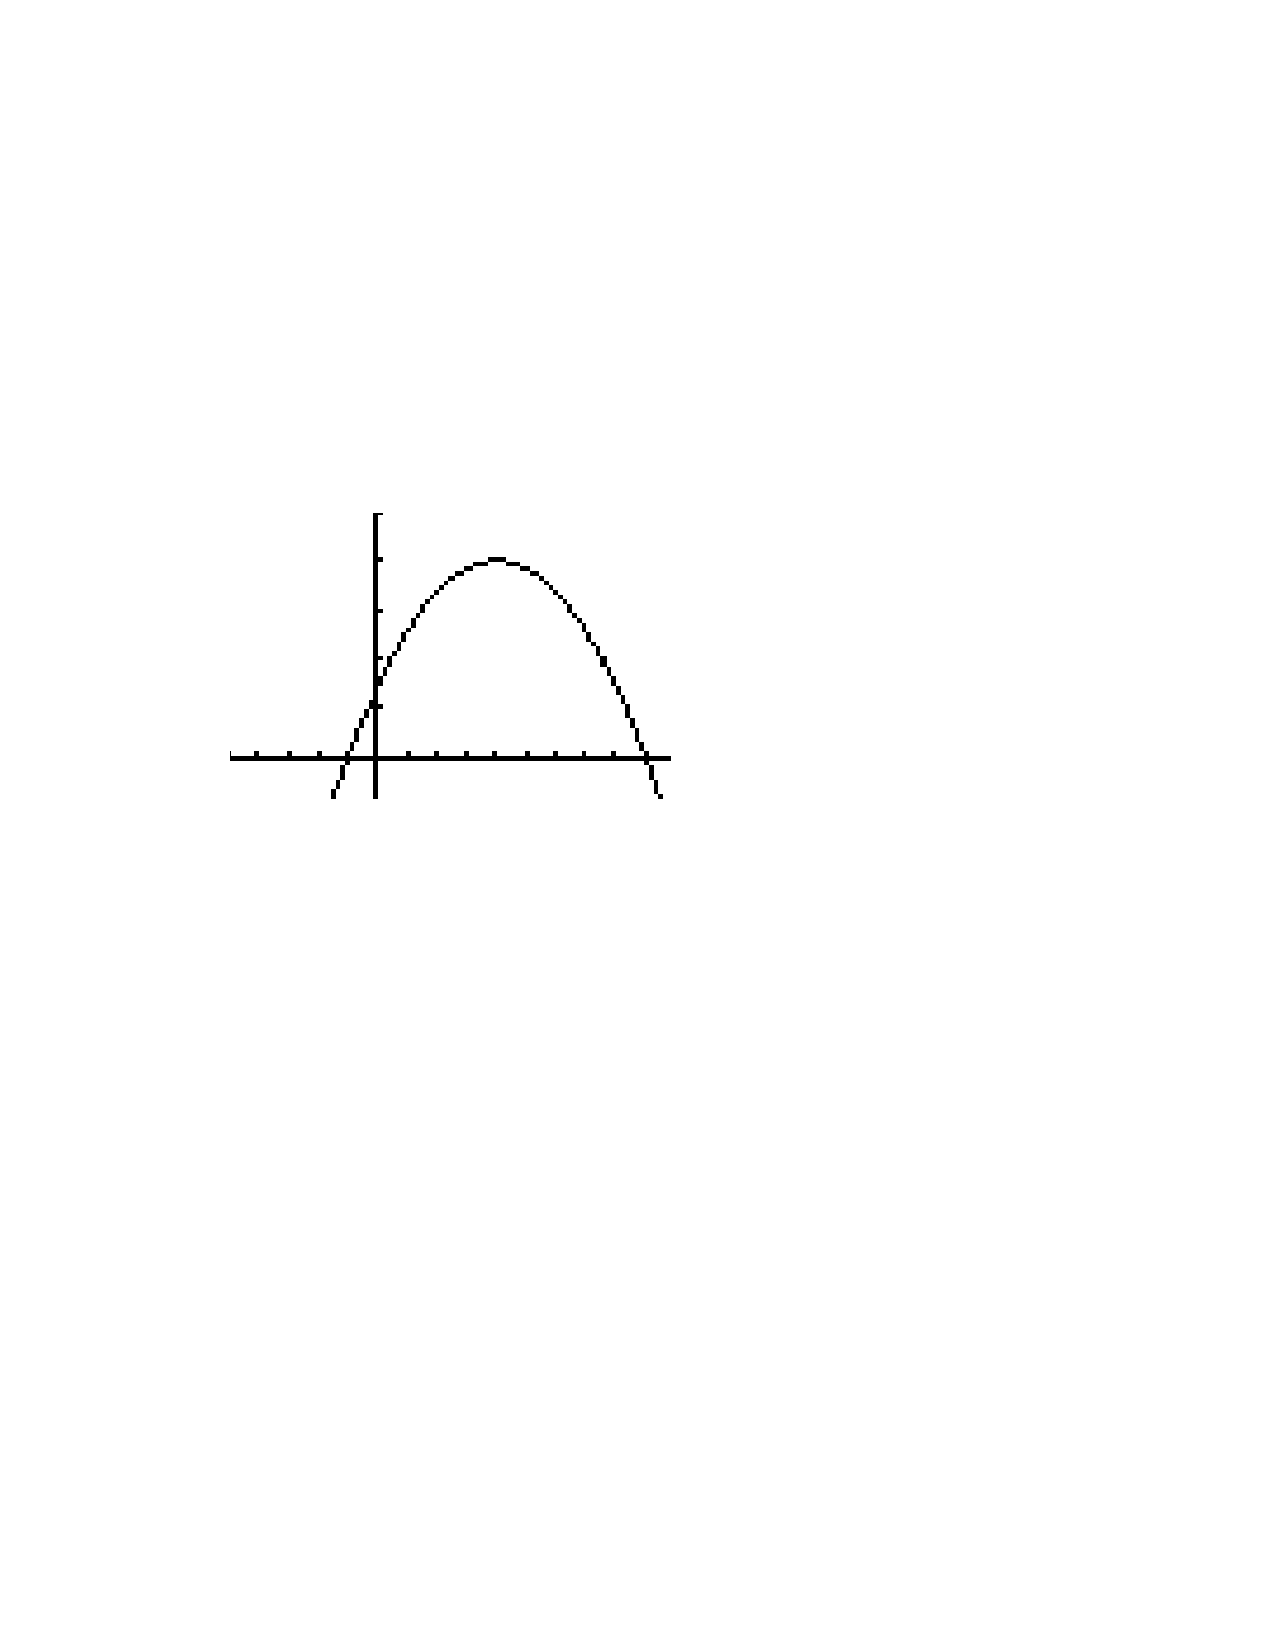
\includegraphics[trim= 250 360 300 185]{Images/Figure1.pdf}
  \end{center}
\end{problem}

\begin{problem}
  \label{problem:find-all-asymptotes}
  \outcome{Recognize when a limit is indicating there is a vertical asymptote.}
  \outcome{Evaluate the limit as $x$ approaches a point where there is a vertical asymptote.}
  \outcome{Discuss what it means for a limit to equal $\pm\infty$.}
  For the function $g$ defined by 
  \[
    g(t) = \frac{t^2 + 7t + 11}{t-3}
  \]
  \begin{itemize}
    \item[(a)]
      Find all vertical asymptotes, (be sure to mention how the function approaches its vertical asymptotes).
      \begin{freeResponse}
        Candidates for vertical asymptote: $t - 3 = 0 \implies t = 3$.

        Test of candidate $t = 3$:
        \begin{align*}
          \lim_{t \to 3^+} \underbrace{\frac{t^2 + 7t + 11}{t-3}}_{\text{from $\text{pos}/0^+$}} &= \infty \\
          &\implies \mbox{vertical asymptote at $t = 3$}
        \end{align*}

        Approach on left-side:
        \begin{align*}
          \lim_{t \to 3^-} \underbrace{\frac{t^2 + 7t + 11}{t-3}}_{\text{from $\text{pos}/0^-$}} &= -\infty \\
          &\implies \mbox{vertical asymptote at $t = 3$}
        \end{align*}
      \end{freeResponse}


    \item[(b)]
      \outcome{Understand the relationship between limits and vertical asymptotes.}
      \outcome{Calculate the limit as $x$ approaches $\pm\infty$ of common functions algebraically.}
      \outcome{Decide whether a form is determinate or indeterminate.}
      Find all horizontal asymptotes.
      \begin{freeResponse}
        \begin{align*}
          \lim_{t \to \infty} \frac{t^2 + 7t + 11}{t-3} \cdot  &= \lim_{t \to \infty} \underbrace{\frac{t + 7 + \frac{11}{t}}{1-\frac{3}{t}}}_\text{form $\infty/\text{pos}$} = \infty \\
          &\implies \mbox{no horizontal asymptotes as $t \to \infty$}
        \end{align*}

        \begin{align*}
          \lim_{t \to -\infty} \frac{t^2 + 7t + 11}{t-3} \cdot  &= \lim_{t \to -\infty} \underbrace{\frac{t + 7 + \frac{11}{t}}{1-\frac{3}{t}}}_\text{form $-\infty/\text{pos}$} = -\infty \\
          &\implies \mbox{no horizontal asymptotes as $t \to -\infty$}
        \end{align*}
      \end{freeResponse}


    \item[(c)]
      Find all slant asymptotes.
      \begin{freeResponse}
        Performing long division:
        \begin{center}
          \includegraphics[scale = 0.3]{"Polynomial division".pdf}
        \end{center}
        we see that
        \[
          \frac{t^2 + 7t + 11}{t-3} = t + 10 + \frac{41}{t-3}.
        \] 
        Thus, $y = x+10$ is a slant asymptote for the graph of $g$.
      \end{freeResponse}
  \end{itemize}
\end{problem}

\subsection*{Extra Problems for for Personal Practice}
\label{section:extra-problems}
% \begin{problem}
%   \label{problem:briggs-2-5-69}
%   Find the vertical and horizontal asymptotes of
%   \[
%     f(x) = \frac{\cos(x) + 2\sqrt{x}}{\sqrt{x}}.
%   \]
% \end{problem}

% \begin{problem}
%   \label{problem:briggs-2-5-82}
%   Use the following instructions to evaluate the given limits of
%   \[
%     f(x) = \frac{e^x + e^{2x}}{e^{2x} + e^{3x}}.
%   \]
%   \begin{itemize}
%     \item[(a)]
%       Evaluate $\displaystyle \lim_{x \to \infty} f(x)$ be dividing both numerator and denominator by $e^{3x}$.

%     \item[(b)]
%       Evaluate $\displaystyle \lim_{x \to -\infty} f(x)$ be dividing both numerator and denominator by $e^{2x}$.

%     \item[(c)]
%       Give the horizontal asymptote(s).

%     \item[(d)]
%       Graph $f$ and confirm your work in parts (a)--(c).
%   \end{itemize}
% \end{problem}

\begin{problem}
  \label{problem:asymptotes}
  \outcome{Recognize when a limit is indicating there is a vertical asymptote.}
  \outcome{Evaluate the limit as $x$ approaches a point where there is a vertical asymptote.}
  For each of the given functions:
  \begin{itemize}
    \item
      find all vertical asymptotes, (be sure to mention how the function approaches its vertical asymptotes)
    \item
      find all horizontal asymptotes,
    \item
      if any, find all points where the function intersects its vertical asymptotes, and
    \item
      if any, find all points where the function intersects its horizontal asymptotes.
  \end{itemize}
  \outcome{Discuss what it means for a limit to equal $\pm\infty$.}
  \outcome{Calculate the limit as $x$ approaches $\pm\infty$ of common functions algebraically.}
  \begin{itemize}
    \item[(a)] The function $f$ defined by $\displaystyle f(x) = \frac{\sqrt{2x^2 + 1}}{3x-5}$.
      \begin{freeResponse}
        Candidate for vertical asymptotes: $3x - 5 = 0 \implies x = 5/3$.

        Test of candidate $x = 5/3$:
        \begin{align*}
          \lim_{x \to \frac{5}{3}^+} \underbrace{\frac{\sqrt{2x^2 + 1}}{3x-5}}_\text{form $\text{pos}/0^+$} &= \infty\\
          &\implies \mbox{vertical asymptote at $x = 5/3$}
        \end{align*}

        \begin{align*}
          \lim_{x \to \frac{5}{3}^-} \underbrace{\frac{\sqrt{2x^2 + 1}}{3x-5}}_\text{form $\text{pos}/0^-$} &= -\infty\\
          &\implies \mbox{vertical asymptote at $x = 5/3$}
        \end{align*}
        
        
        Test of horizontal asymptote as $x \to \infty$:
        \begin{align*}
          \lim_{x \to \infty} \frac{\sqrt{2x^2 + 1}}{3x-5}
          &= \lim_{x \to \infty} \frac{\sqrt{2x^2 + 1}}{3x-5} \cdot \frac{\frac{1}{x}}{\frac{1}{x}} \\
          &= \lim_{x \to \infty}  \frac{\frac{\sqrt{2x^2 + 1}}{\sqrt{x^2}}}{3 - \frac{5}{x}}\\
          &= \lim_{x \to \infty}  \frac{\sqrt{2 + \frac{1}{x^2}}}{3 - \frac{5}{x}} \\
          &= \frac{\sqrt{2}}{3} \\
          &\implies \mbox{horizontal asymptote $y = \sqrt{2}/3$ as $x \to \infty$}
        \end{align*}

        Test of horizontal asymptote as $x \to -\infty$:
        \begin{align*}
          \lim_{x \to -\infty} \frac{\sqrt{2x^2 + 1}}{3x-5}
          &= \lim_{x \to -\infty} \frac{\sqrt{2x^2 + 1}}{3x-5} \cdot \frac{\frac{1}{x}}{\frac{1}{x}} \\
          &= \lim_{x \to -\infty}  \frac{\frac{\sqrt{2x^2 + 1}}{-\sqrt{x^2}}}{3 - \frac{5}{x}}\\
          &= \lim_{x \to -\infty}  \frac{-\sqrt{2 + \frac{1}{x^2}}}{3 - \frac{5}{x}} \\
          &= \frac{-\sqrt{2}}{3} \\
          &\implies \mbox{horizontal asymptote $y = -\sqrt{2}/3$ as $x \to -\infty$}
        \end{align*}

        Graph intersects vertical asymptote?

        No: both right-sided and left-sided limits as $x \to 5/3$ don't exist.

        Graph intersects horizontal asymptote $y = \sqrt{2}/3$?
        
        No:
        \begin{align*}
          \frac{\sqrt{2x^2 + 1}}{3x-5} = \frac{\sqrt{2}}{3} &\implies 3 \sqrt{2x^2+1} = \sqrt{2}(3x-5)\\
          &\implies 9 (2x^2 + 1) = 2(9x^2 - 30x + 25) \\
          &\implies x = \frac{41}{60}\\
          &\implies f(41/60) = - \sqrt{2}/3\\
          &\implies \mbox{$x = 41/60$ is an extraneous solution}
        \end{align*}

        Graph intersects horizontal asymptote $y = -\sqrt{2}/3$?
        
        Yes:
        \begin{align*}
          \frac{\sqrt{2x^2 + 1}}{3x-5} = \frac{-\sqrt{2}}{3}
          &\implies 3 \sqrt{2x^2+1} = -\sqrt{2}(3x-5)\\
          &\implies x = \frac{41}{60}\\
          &\implies f(41/60) = - \sqrt{2}/3\\
          &\implies \mbox{graph of $f$ intersects $y = -\sqrt{2}/3$ at $x = 41/60$}
        \end{align*}
      \end{freeResponse}


    \item[(b)] The function $s$ defined by $\displaystyle s(t) = \sqrt{t^2 + 8t + 1} - t$.
      \begin{freeResponse}
        Finding domain of $s$:
        \[
          t^2 + 8t + 1 \ge 0 \implies t = -4 \pm \sqrt{15}
        \]
        Sign chart:
        \begin{image}
          \includegraphics[scale = 0.1]{Images/"Number line to determine domain".png}
        \end{image}
      \end{freeResponse}
      So the domain of $s$ is $(-\infty, -4 -\sqrt{15}] \cup [-4+\sqrt{15}, \infty)$.

      Candidate for vertical asymptotes: by limit laws, $\lim_{x \to a} s(t) = s(a)$ for any $a$ in $(-\infty, -4 -\sqrt{15}) \cup (-4+\sqrt{15}, \infty)$, $\lim_{x \to (-4 -\sqrt{15})^-} s(t) = s(-4 -\sqrt{15})$, and $\lim_{x \to (-4 +\sqrt{15})^+} s(t) = s(-4 +\sqrt{15})$ implies no candidates for vertical asymptotes.

      Test of horizontal asymptote as $x \to \infty$:
      \begin{align*}
        \lim_{t \to \infty} \sqrt{t^2 +  8t + 1} - t
        &= \lim_{t \to \infty} (\sqrt{t^2 + 8t + 1} - t) \cdot \frac{\sqrt{t^2 + 8t + 1} + t}{\sqrt{t^2 + 8t + 1} + t}\\
          &= \lim_{t \to \infty} \frac{t^2 + 8t + 1 - t^2}{\sqrt{t^2 + 8t + 1} + t}\\
          &= \lim_{t \to \infty} \frac{8t + 1}{\sqrt{t^2 + 8t + 1} + t} \cdot \frac{\frac{1}{t}}{\frac{1}{t}} \\
          &= \lim_{t \to \infty} \frac{8 + 1/t}{\sqrt{1 + 8/t + 1/t^2} + 1} = 8/2 = 4\\
        &\implies \mbox{horizontal asymptote $y = 4$ as $t \to \infty$}
        \end{align*}

      No vertical asymptotes implies no intersection points on vertical asymptotes.

      Test of horizontal asymptote as $x \to -\infty$:
      \begin{align*}
        \lim_{t \to -\infty} \sqrt{t^2 +  8t + 1} - t
        &= \lim_{t \to -\infty} (\sqrt{t^2 + 8t + 1} - t) \cdot \frac{\sqrt{t^2 + 8t + 1} + t}{\sqrt{t^2 + 8t + 1} + t}\\
          &= \lim_{t \to -\infty} \frac{t^2 + 8t + 1 - t^2}{\sqrt{t^2 + 8t + 1} + t}\\
          &= \lim_{t \to -\infty} \frac{8t + 1}{\sqrt{t^2 + 8t + 1} + t} \cdot \frac{\frac{1}{t}}{\frac{1}{t}} \\
          &= \lim_{t \to -\infty} \frac{8 + 1/t}{-\sqrt{1 + 8/t + 1/t^2} - t/\sqrt{t^2}}\\
        &= \lim_{t \to -\infty} \underbrace{\frac{8 + 1/t}{-\sqrt{1 + 8/t + 1/t^2} +1}}_\text{form $8/0^+$} = \infty\\
        &\implies \mbox{no horizontal asymptotes as $t \to -\infty$}
        \end{align*}
        
     Intersection points on horizontal asymptote:
     \begin{align}
       \sqrt{t^2 + 8t + 1} - t = 4 &\implies \sqrt{t^2 + 8t + 1} = 4 + t\\
       &\implies t^2 + 8t + 1 = (4 + t)^2 = 16 + 8t + t^2\\
       &\implies 1 = 16 \implies \mbox{no intersection points with horizontal asymptote}
     \end{align}
  \end{itemize}
\end{problem}

\begin{problem}
  \label{problem:sketch-a-graph}
  \outcome{Recognize when a limit is indicating there is a vertical asymptote.}
  \outcome{Discuss what it means for a limit to equal $\pm\infty$.}
  \outcome{Define a vertical asymptote.}
  \outcome{Understand the relationship between limits and vertical asymptotes.}
  \outcome{Discuss why infinity is not a number.}
  Sketch the graph of a function that satisfies all of the given properties.
  (You \emph{do not} need to find a formula for the function.)
  \begin{center}
    \begin{tabular}[c]{llll}
      \toprule
      & & \hspace{-5em}Required Properties\\
      \midrule
      $\displaystyle \lim_{x \to -2^-} f(x) = \infty$ & $f(-2) = 7$ & $f(1) = 2$ & $\displaystyle \lim_{x \to \infty} f(x) = 3$ \\
      $\displaystyle \lim_{x \to -\infty} f(x) = -\infty$ & $\lim_{x \to 5} f(x) = \infty$ & $\displaystyle \lim_{x \to 9} f(x) = 3$ & $f(9) = 1$\\
      $\displaystyle \lim_{x \to -3^-} f(x) = \infty$ & $\displaystyle \lim_{x \to -3^+} f(x) = -\infty$ & $f(4) \text{ is undefined, }$ & $f(x) = 3 \text{ for } x>9$\\
      \bottomrule
    \end{tabular}
  \end{center}
  \begin{freeResponse}
      There are many correct solutions to this problem.
  One possible solution can be constructed as follows:
  \begin{center}
    \includegraphics[scale = 0.3]{Images/"Drawing graph with given properties 1".pdf}
  \end{center}
    \begin{center}
    \includegraphics[scale = 0.3]{Images/"Drawing graph with given properties 2".pdf}
  \end{center}
  \begin{center}
    \includegraphics[scale = 0.3]{Images/"Drawing graph with given properties 3".pdf}
  \end{center}
  \begin{center}
    \includegraphics[scale = 0.3]{Images/"Drawing graph with given properties 4".pdf}
  \end{center}
  \end{freeResponse}

\end{problem}
\end{document} 
